\chapter*{Appendix}

\renewcommand{\thefigure}{A.\arabic{figure}}
\setcounter{figure}{0}

\begin{figure}[h!]
    \centering

    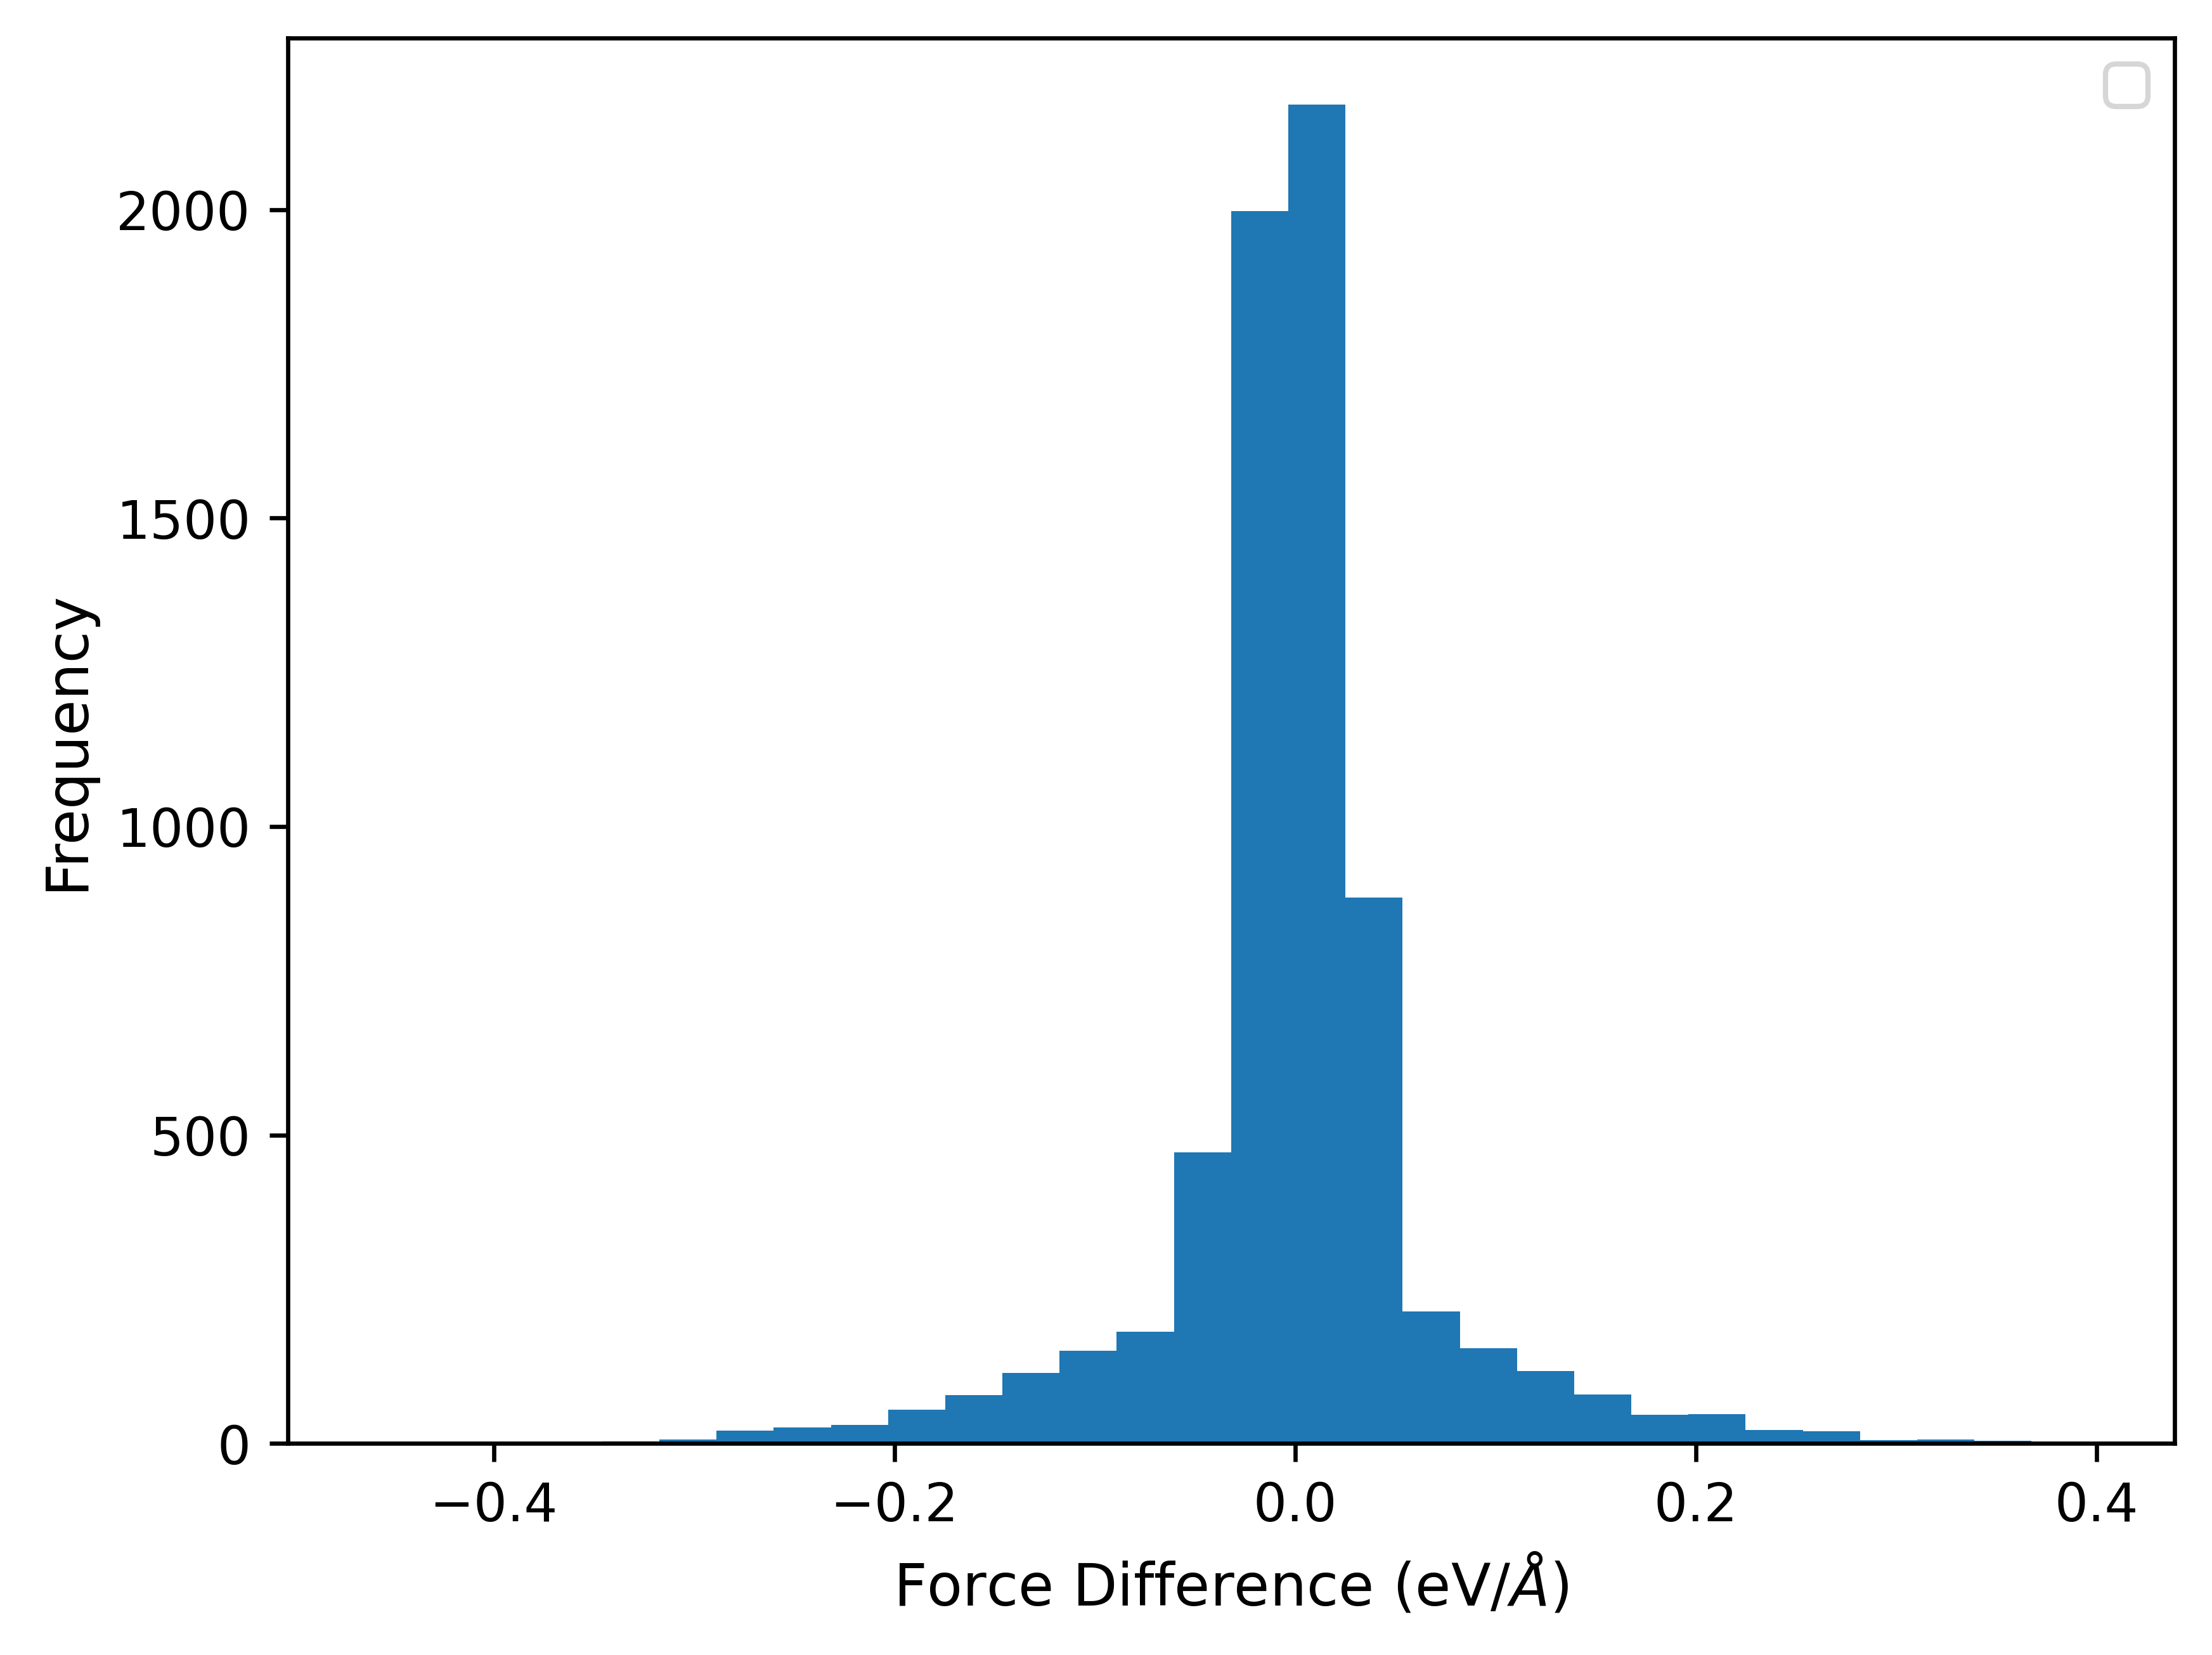
\includegraphics[width=0.6\linewidth]{images/scan_vs_r2scan/r2scan_hist_force.png}
    \caption{Distribution of the error on forces between SCAN and r2SCAN
        functional.
    }
    \label{fig:scan_r2scan_F_dist}
\end{figure}

\begin{figure}[tbhp]
    \centering
    \begin{subfigure}{0.32\textwidth}
        \centering
        \includegraphics[width=1\textwidth]{convergence/SCAN/conv-energy.png}
        \caption{}
        % \label{fig:}
    \end{subfigure}
    \hfill
    \begin{subfigure}{0.32\textwidth}
        \centering
        \includegraphics[width=1\textwidth]{convergence/SCAN/conv-force.png}
        \caption{}
        % \label{fig:}
    \end{subfigure}
    \hfill
    \begin{subfigure}{0.32\textwidth}
        \centering

        \includegraphics[width=1\textwidth]{convergence/SCAN/conv-pressure.png}
        \caption{}
        % \label{fig:}
    \end{subfigure}
    \caption{Convergence tests using the SCAN functional on (a) total energy,
        (b) total force, and (c) total pressure. All values are shifted
        with respect to the reference value at 180 Ry. The forces and pressure
        are also normalized with the corresponding reference values at 180 Ry.}
    \label{fig:conv_scan}
\end{figure}

\begin{figure}[tbhp]
    \centering
    \begin{subfigure}{0.32\textwidth}
        \centering
        \includegraphics[width=1\textwidth]{convergence/R2SCAN/conv-energy.png}
        \caption{}
        % \label{fig:}
    \end{subfigure}
    \hfill
    \begin{subfigure}{0.32\textwidth}
        \centering
        \includegraphics[width=1\textwidth]{convergence/R2SCAN/conv-force.png}
        \caption{}
        % \label{fig:}
    \end{subfigure}
    \hfill
    \begin{subfigure}{0.32\textwidth}
        \centering

        \includegraphics[width=1\textwidth]{convergence/R2SCAN/conv-pressure.png}
        \caption{}
        % \label{fig:}
    \end{subfigure}
    \caption{Convergence tests using the r$^2$SCAN functional on (a) total
        energy,
        (b) total force, and (c) total pressure.  All values are shifted
        with respect to the reference value at 180 Ry. The forces and pressure
        are also normalized with the corresponding reference values at 180 Ry.}
    \label{fig:conv_r2scan}
\end{figure}

\begin{figure}[h!]
    \centering
    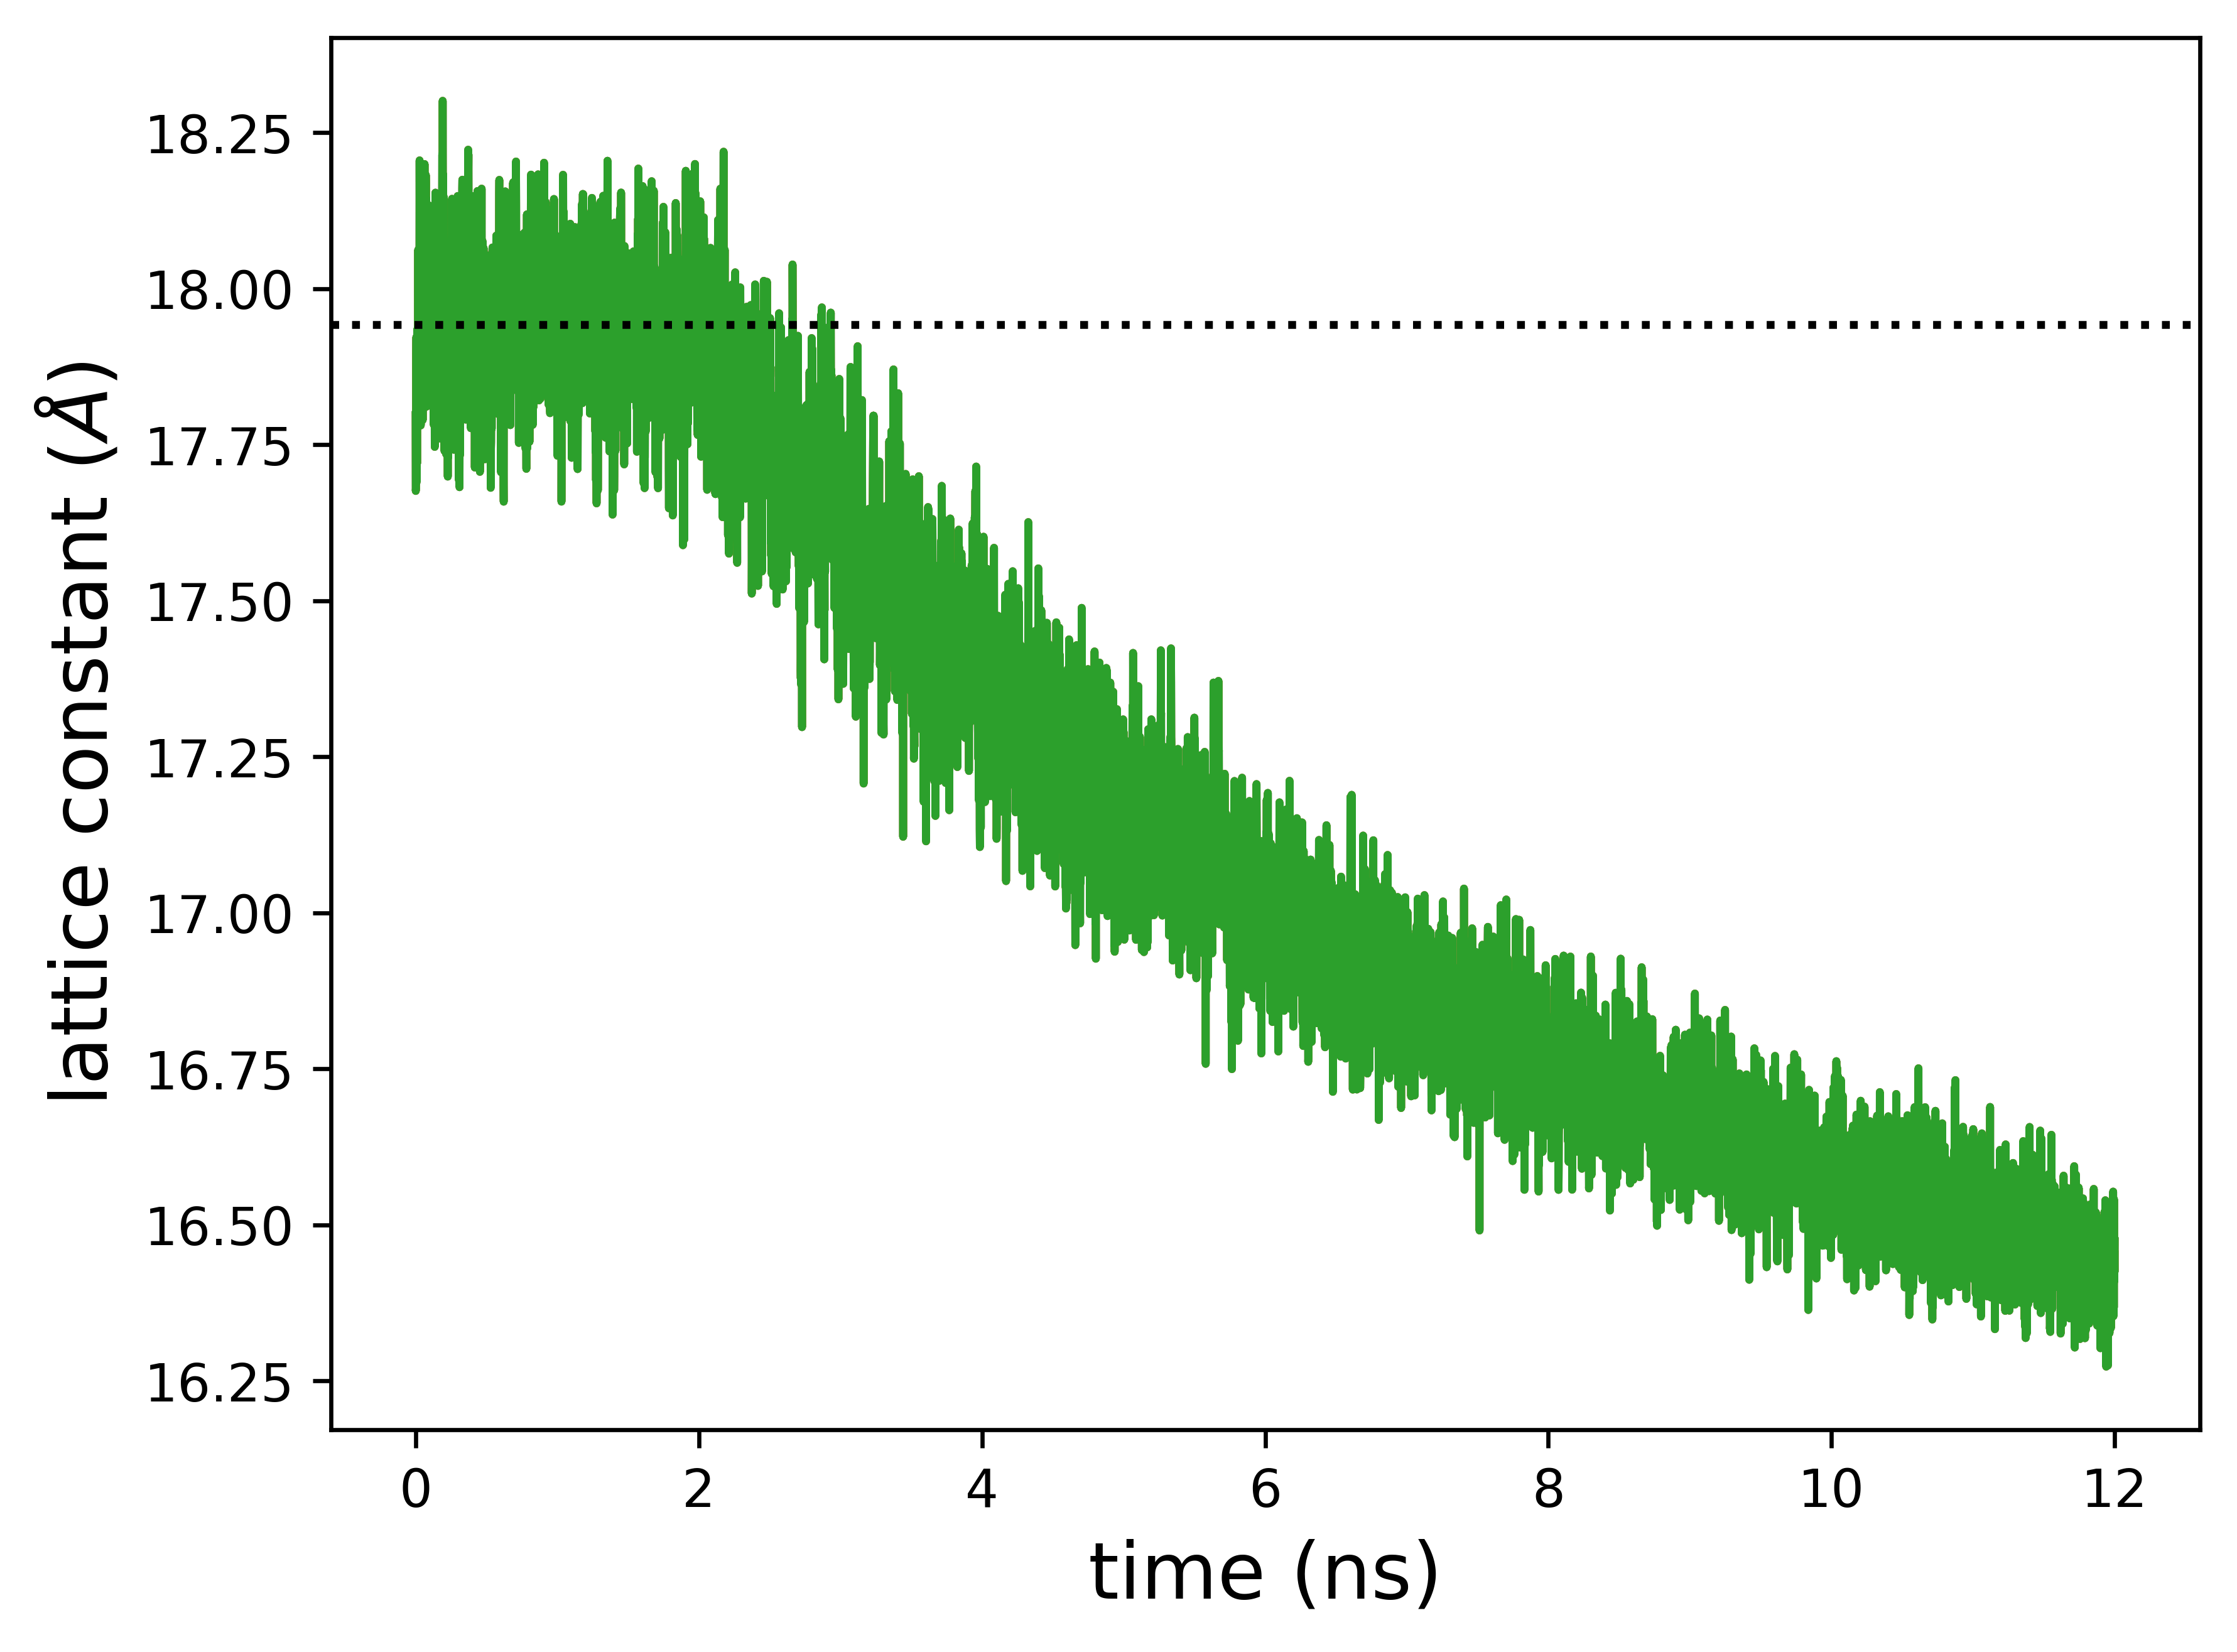
\includegraphics[width=0.4\linewidth]{images/330K/conv-lattice.png}
    \caption{Lattice parameter as a function of simulation steps. }
\end{figure}